\chapter*{Symbols Table}
%\addcontentsline{toc}{chapter}{\textcolor{ocre}{Symbols Table}}

This appendix contains the description of reserved keywords and of the operators of B language, sorted by ascending ASCII order.\\
For each reserved keyword or operator, this chapter provides:
\begin{itemize}
    \item its \textbf{ASCII notation}, 
    \item its \textbf{mathematical notation}, if it differs from its ASCII notation.
    \item its \textbf{priority level}. The priority level corresponds to the priority level during the syntactic analysis. The higher the priority level of an operator, the more it attracts operands. For example, if the operators op40 and op250 are respectively of 40 and 250 priority, then the expression x op40 y op250 z is analysed as x op40 (y op250 z)
    \item its \textbf{associative properties} (L for associative to the left or R for associative to the right). If two binary operators named op have the same priority, then: x op y op z will be analysed as (x op y) op z if op is associative to the left; and as x op (y op z) if op is associative to the right.
    \item its \textbf{description}.
\end{itemize}
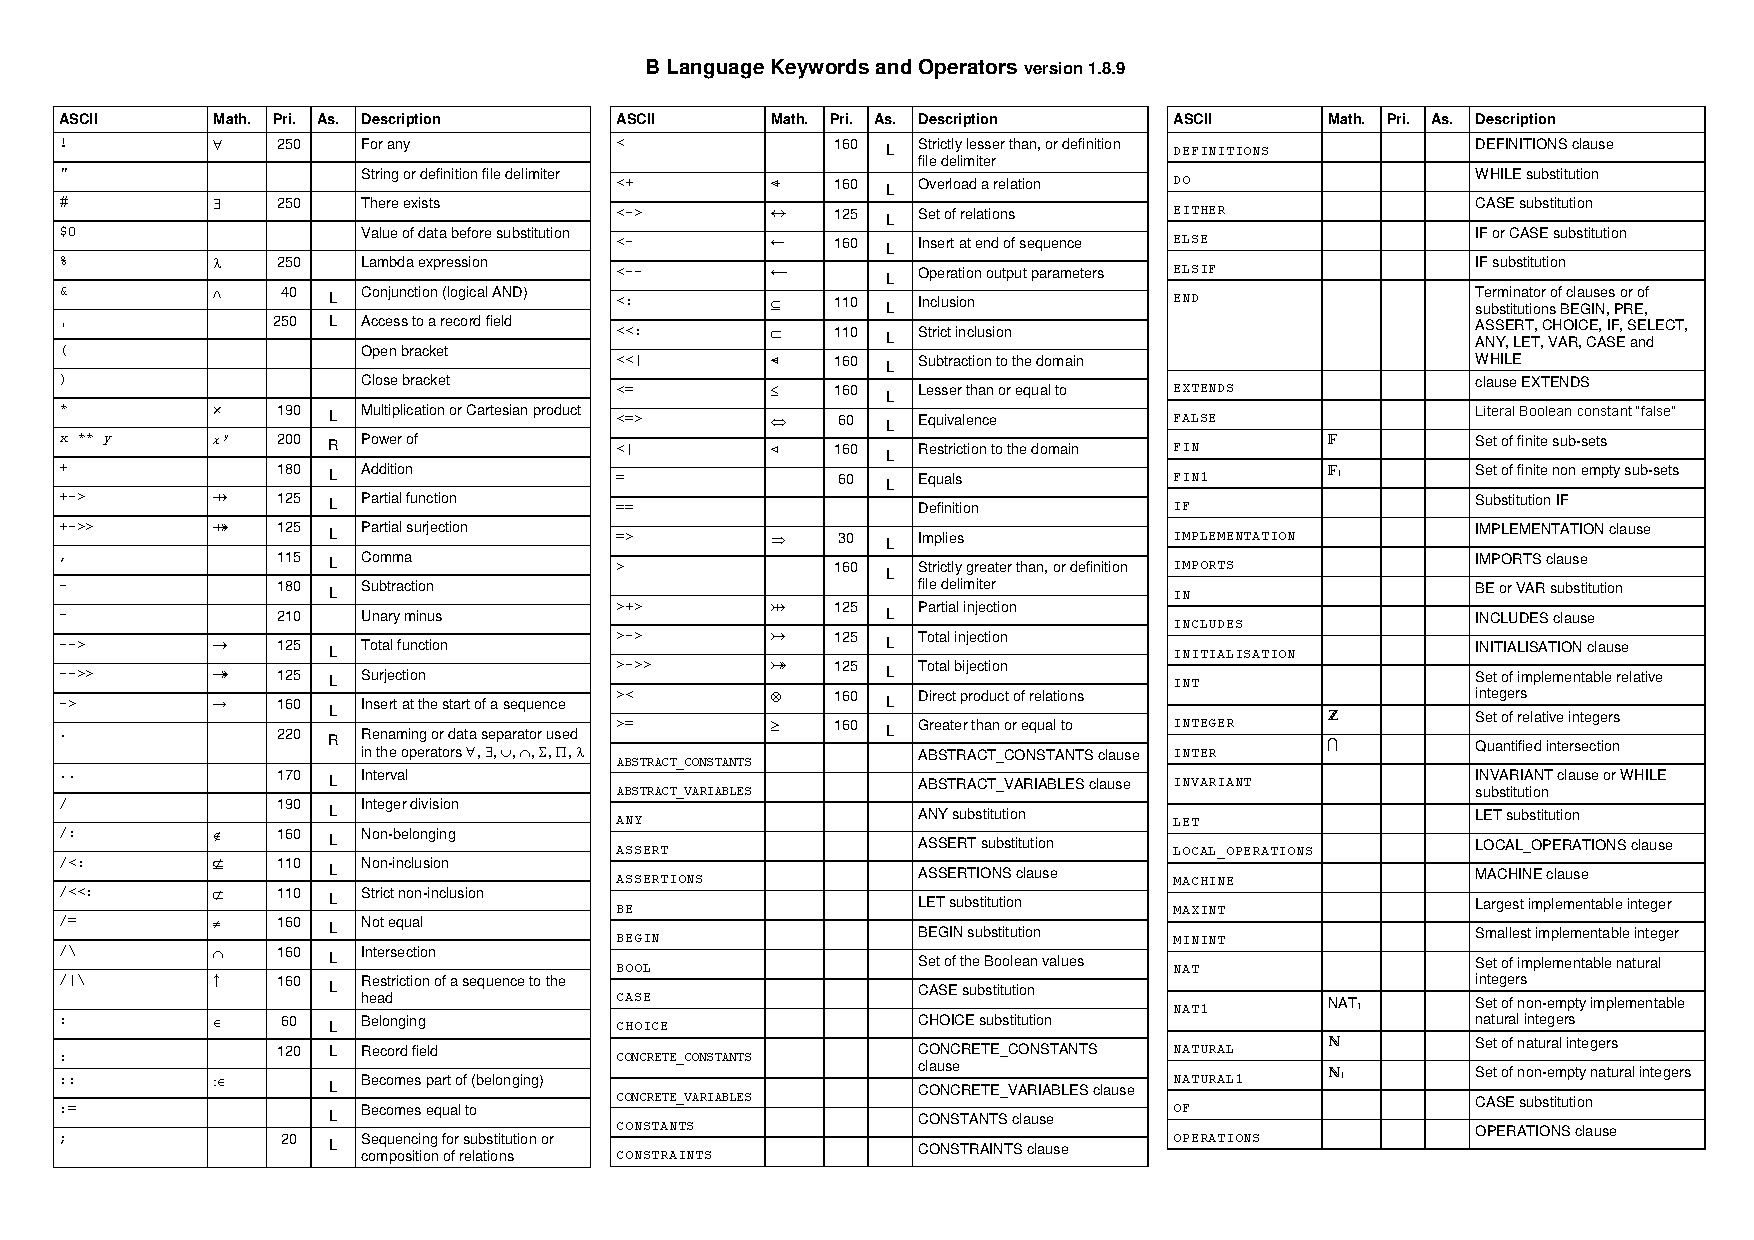
\includepdf[pages={1},landscape=true]{symboles-uk}
\includepdf[pages={2},landscape=true]{symboles-uk}